%%%%%%%%%%%%%%%%%%%%%%%%%%%%%%%%%%%%%
%% frame
%%%%%%%%%%%%%%%%%%%%%%%%%%%%%%%%%%%%%%
\begin{frame}[t]
	\frametitle{Experimental Results: Filter}
	\framesubtitle{~~}  %% needed for proper positioning of the logo ...

	\begin{figure}[h] \centering
		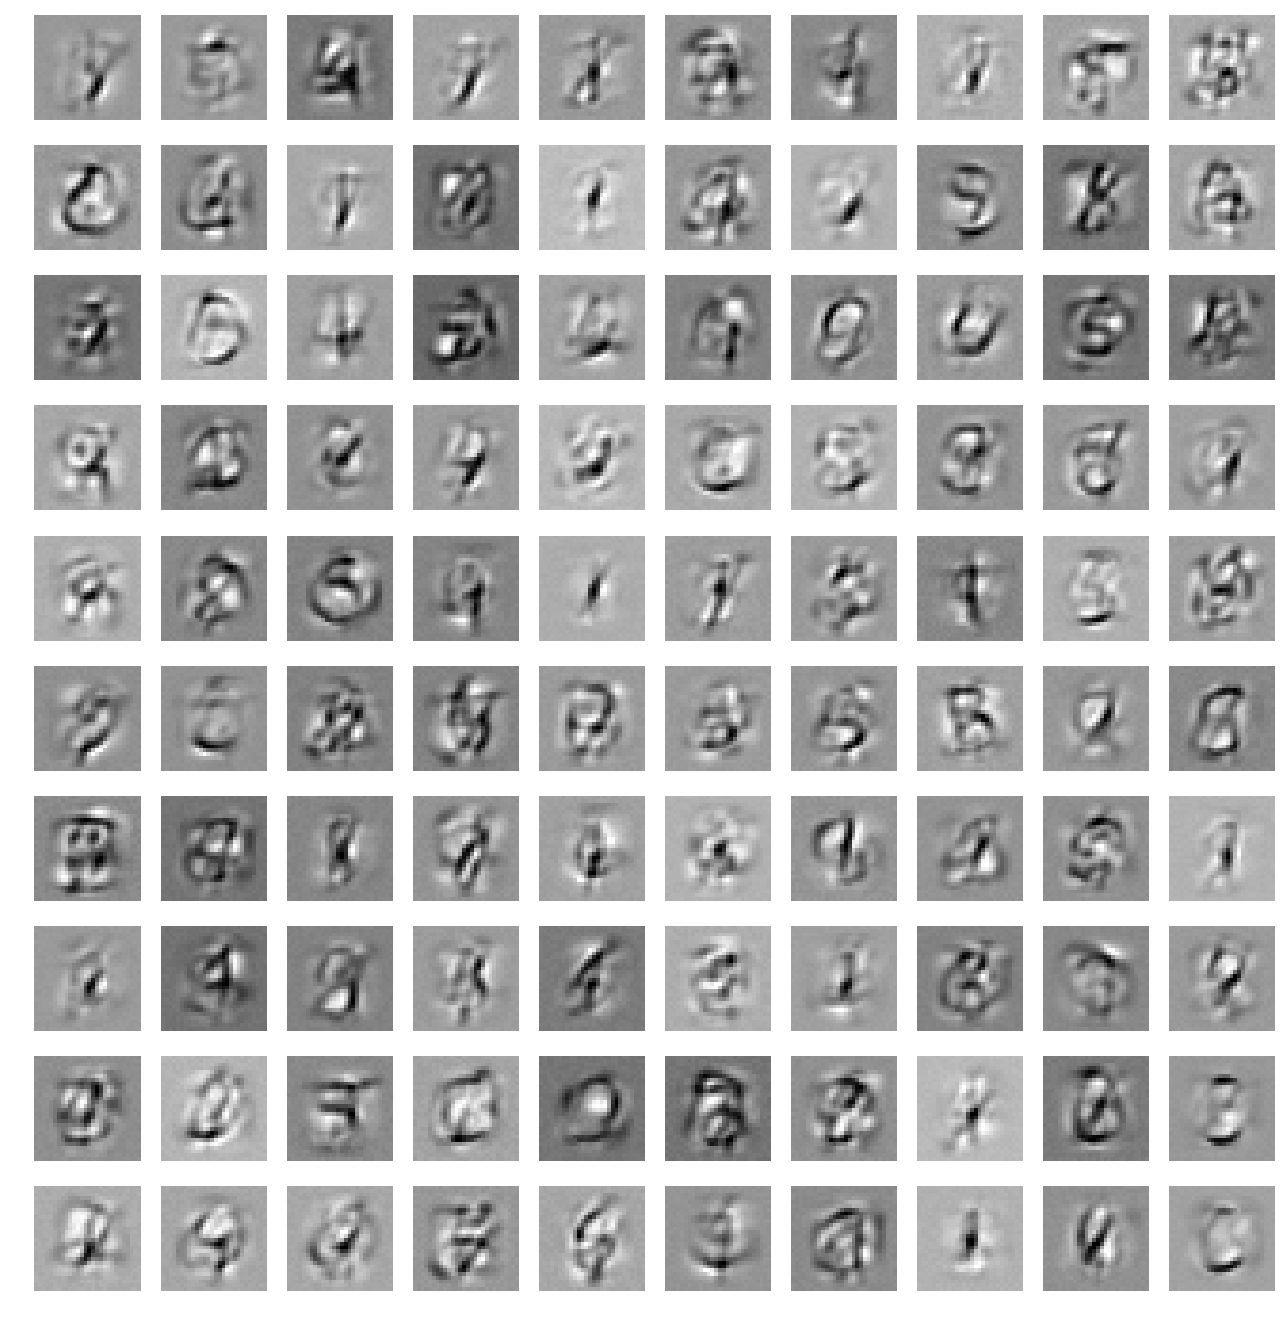
\includegraphics[width=0.45\linewidth]{experiment3_1.png}
		\caption{Visualization of the filters of the first 100 hidden nodes in an
		denoising autoencoder trained over all 60000 images.}
		\label{fig:experiment3_1}
	\end{figure}

\end{frame}
%%%%%%%%%%%%%%%%%%%%%%%%%%%%%%%%%%%%%
%% Frame
%%%%%%%%%%%%%%%%%%%%%%%%%%%%%%%%%%%%%%
\begin{frame}[t]
	\frametitle{Experimental Results: Reconstructing}
	\framesubtitle{~~}  %% needed for proper positioning of the logo ...

\begin{figure}
  \centering
  \subfloat[]{
    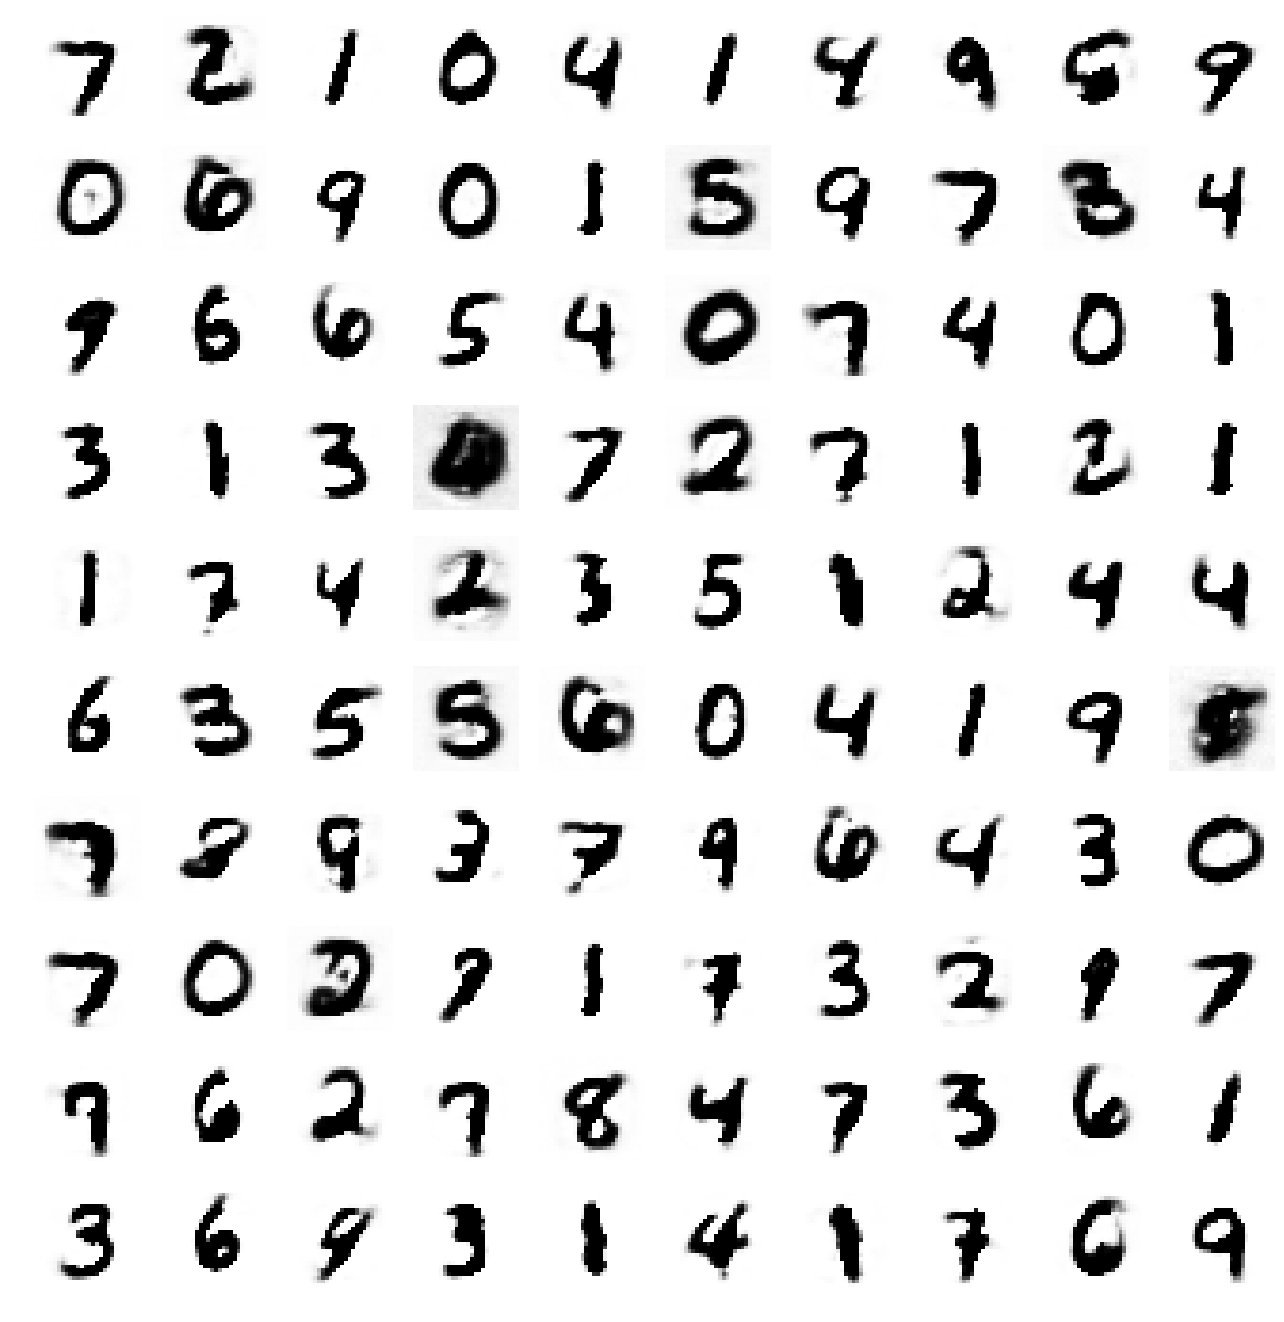
\includegraphics[width=0.4\linewidth]{experiment3_2.png}
  }
  \subfloat[]{
    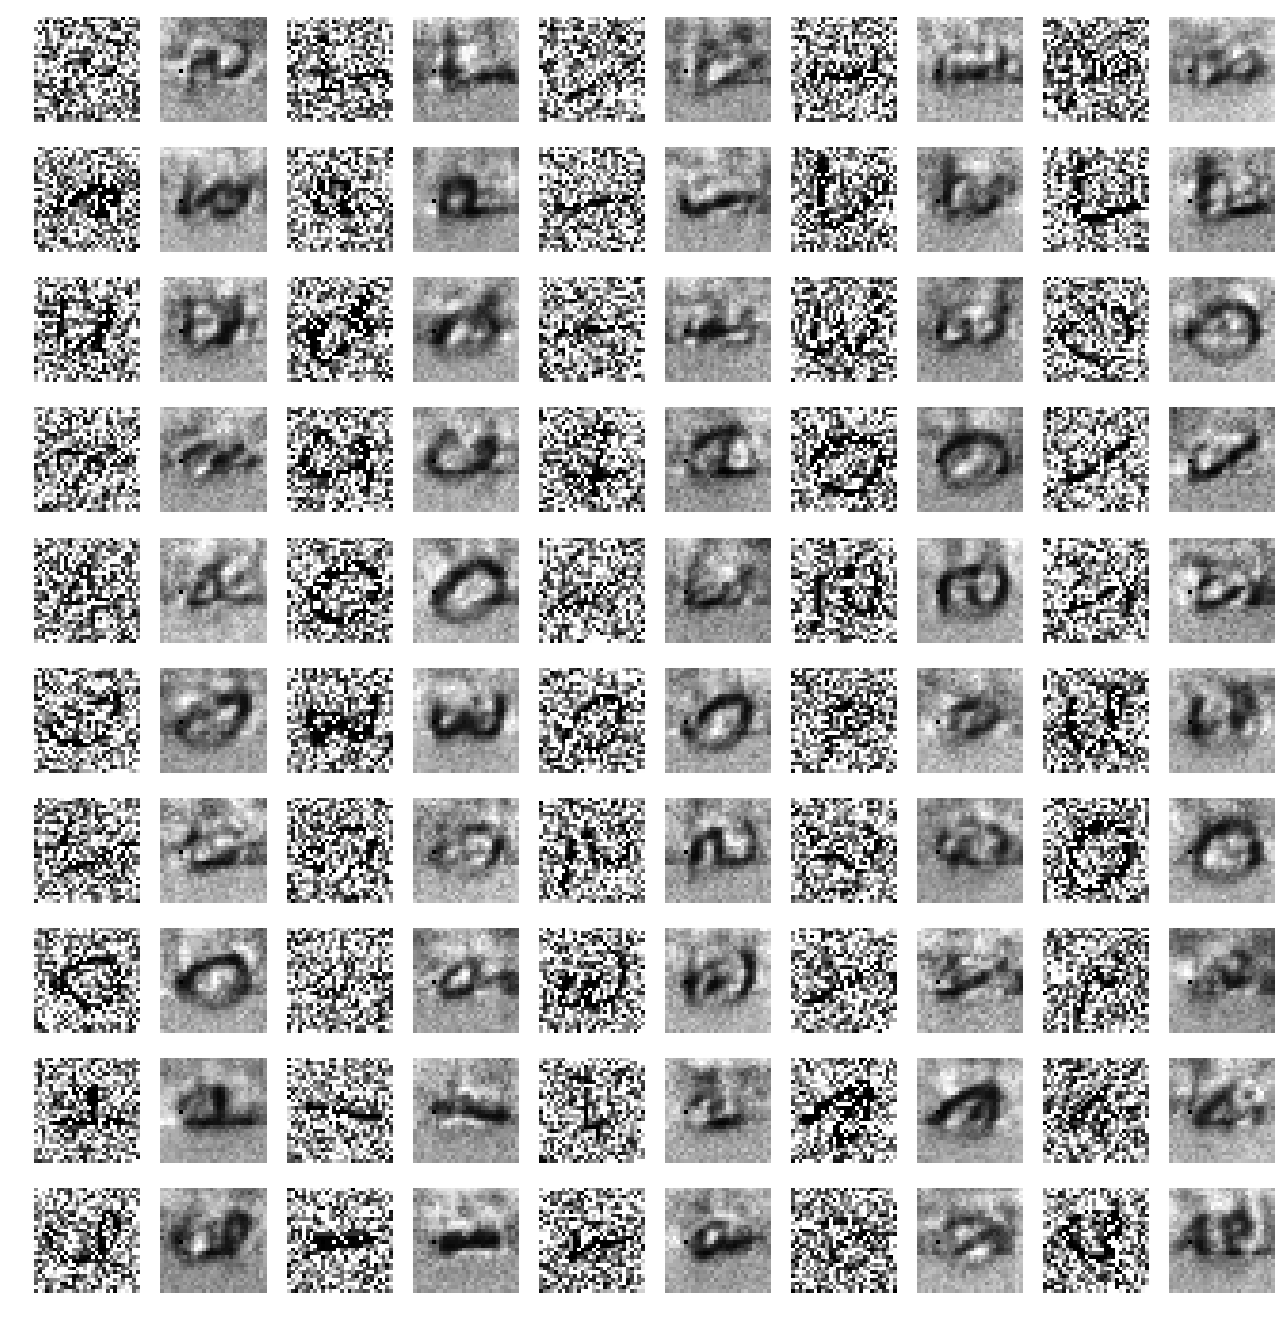
\includegraphics[width=0.4\linewidth]{rand.png}
  }
  \caption{Reconstructions of corrupted digits from the (a) MNIST dataset and  (b) bg-rand dataset}
  \label{fig:reconstruct}
\end{figure}

\end{frame}


%%%%%%%%%%%%%%%%%%%%%%%%%%%%%%%%%%%%%
%% frame
%%%%%%%%%%%%%%%%%%%%%%%%%%%%%%%%%%%%%%
\begin{frame}[t]
	\frametitle{Experimental Results: Reconstructing}
	\framesubtitle{~~}  %% needed for proper positioning of the logo ...

\begin{figure}
  \centering
  \subfloat[]{
    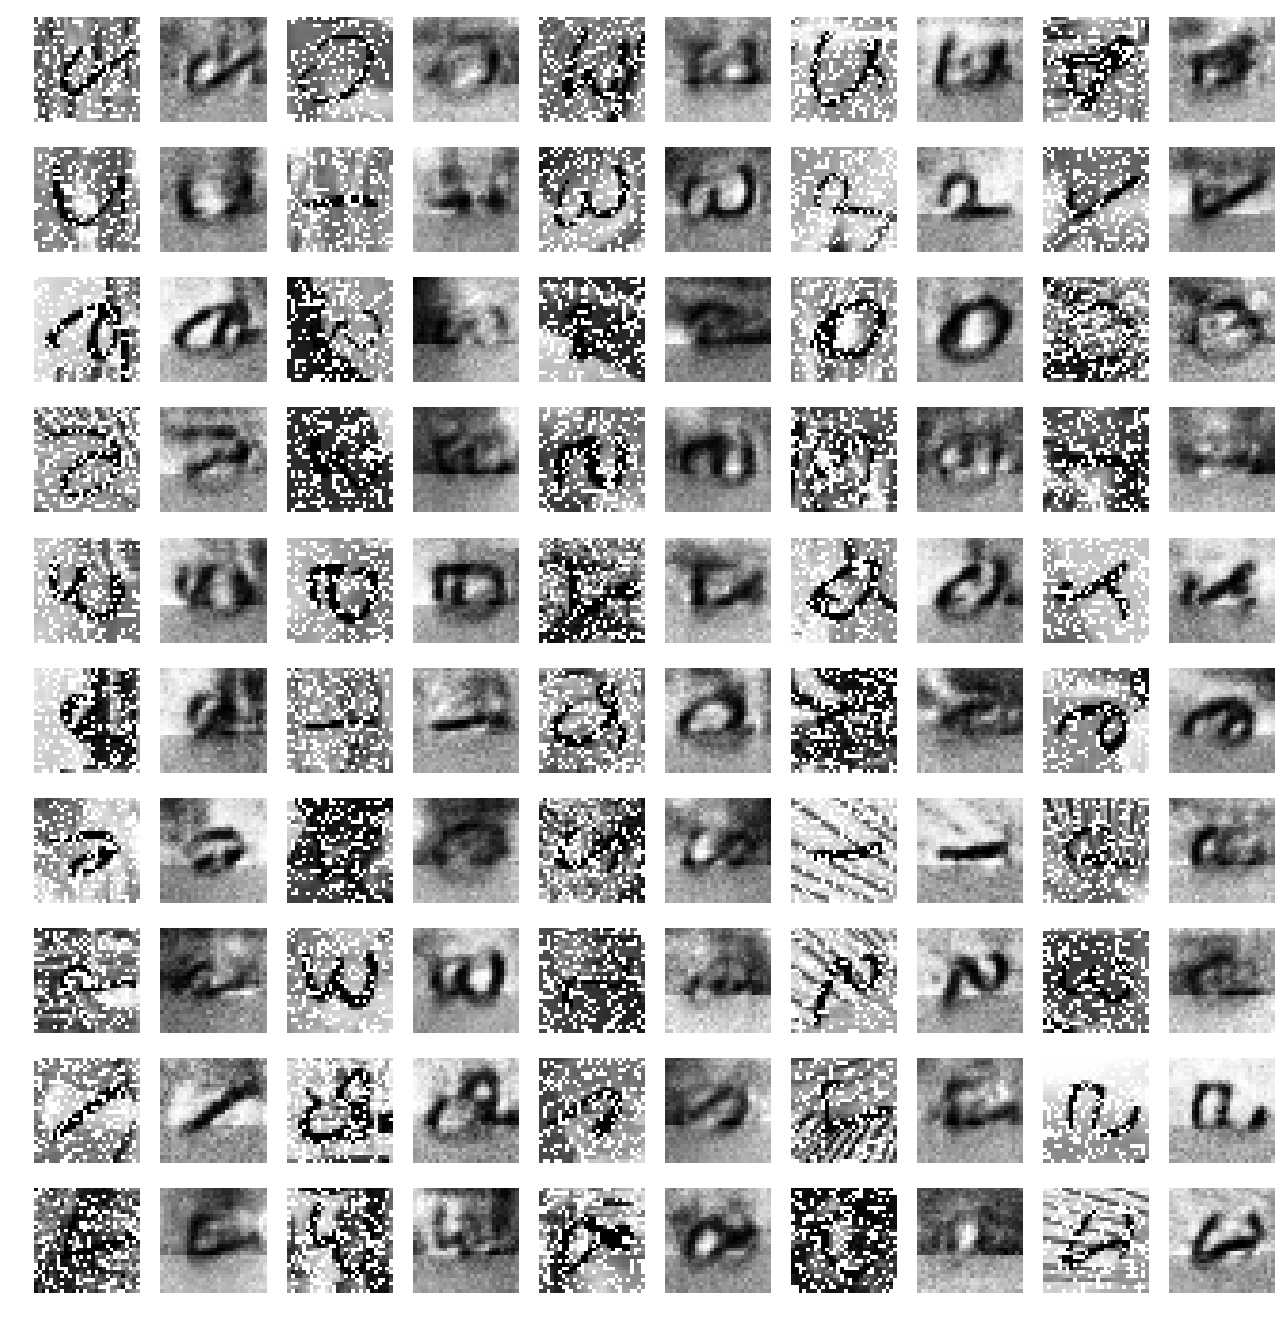
\includegraphics[width=0.4\linewidth]{bg.png}
  }
  \subfloat[]{
    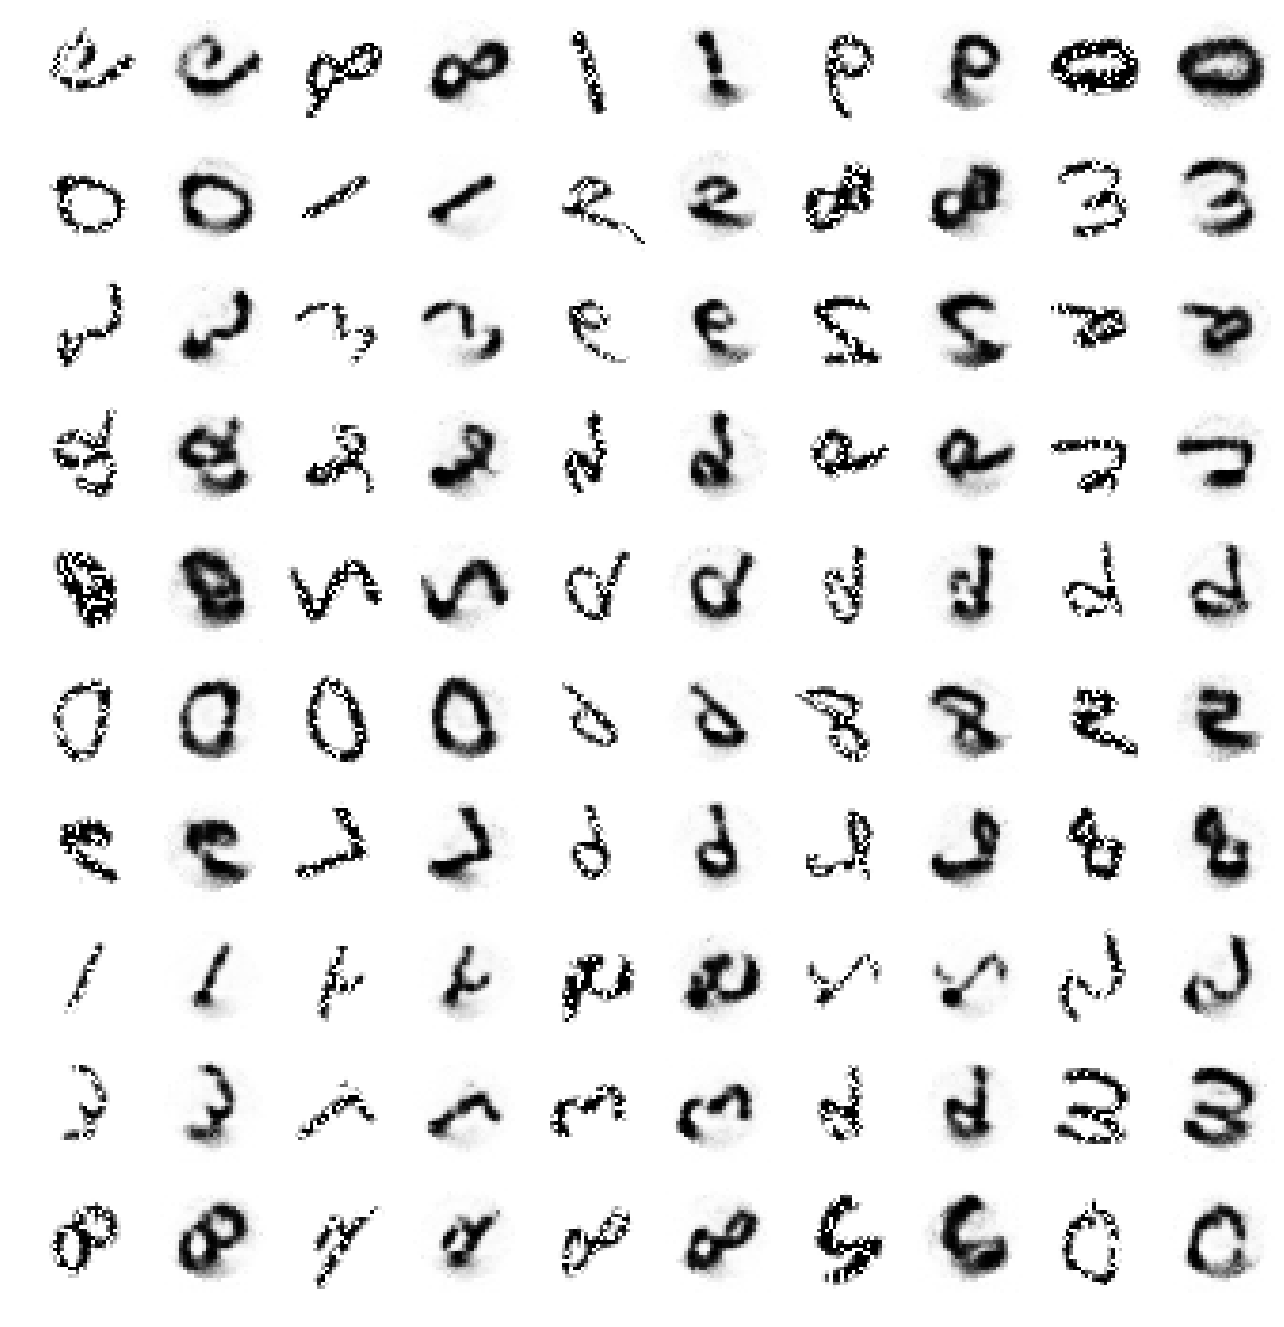
\includegraphics[width=0.4\linewidth]{rot.png}
  }
  \caption{Reconstructions of corrupted digits from the (a) bg-img dataset and (b) rot dataset}
  \label{fig:reconstruct}
\end{figure}

\end{frame}

%%%%%%%%%%%%%%%%%%%%%%%%%%%%%%%%%%%%%
%% Frame
%%%%%%%%%%%%%%%%%%%%%%%%%%%%%%%%%%%%%%
\begin{frame}[t]
	\frametitle{Experimental Results: Supervised Learning}
	\framesubtitle{~~}  %% needed for proper positioning of the logo ...


\begin{table}[h]
  \centering
\begin{tabular}{ll|lll}
    Dataset                        & Data               & Linear SVM & Kernel SVM (RBF) & Logistic Regression \\ \hline
    \multirow{2}{*}{MNIST}         & Original           & 91.68\%    & 94.46\%          & 91.82\%             \\
                                   & Encoded            & 97.07\%    & 95.48\%          & 96.86\%             \\ \hline
    \multirow{2}{*}{mnist-bg-rand} & Original           & 58.975\%   & 83.875\%         & 65.5917\%           \\
                                   & Encoded            & 81.675\%   & 83.6583\%        & 83.825\%            \\ \hline
    \multirow{2}{*}{mnist-bg-img}  & Original           & 69.25\%    & 76.4667\%        & 71.6333\%           \\
                                   & Encoded            & 78.4333\%  & 72.8417\%        & 78.1333\%           \\ \hline
    \multirow{2}{*}{mnist-rot}     & Original           & 11.204\%   & 13.328\%         & 11.868\%           \\
                                   & Encoded            & 18.428\%   & 14.378\%         & 18.78\%
\end{tabular}
  \caption{Summary of the results of running different classification algorithms on the raw MNIST data and on the output from a trained autoencoder. We
  see in all cases that using the encoded data produces a better result.}
  \label{tab:classvsenc}
\end{table}

\end{frame}

%%%%%%%%%%%%%%%%%%%%%%%%%%%%%%%%%%%%%
%% Frame
%%%%%%%%%%%%%%%%%%%%%%%%%%%%%%%%%%%%%%
\begin{frame}[t]
	\frametitle{Experimental Results: SGD Performance}
	\framesubtitle{~~}  %% needed for proper positioning of the logo ...
	\begin{figure}[h]
		\centering
		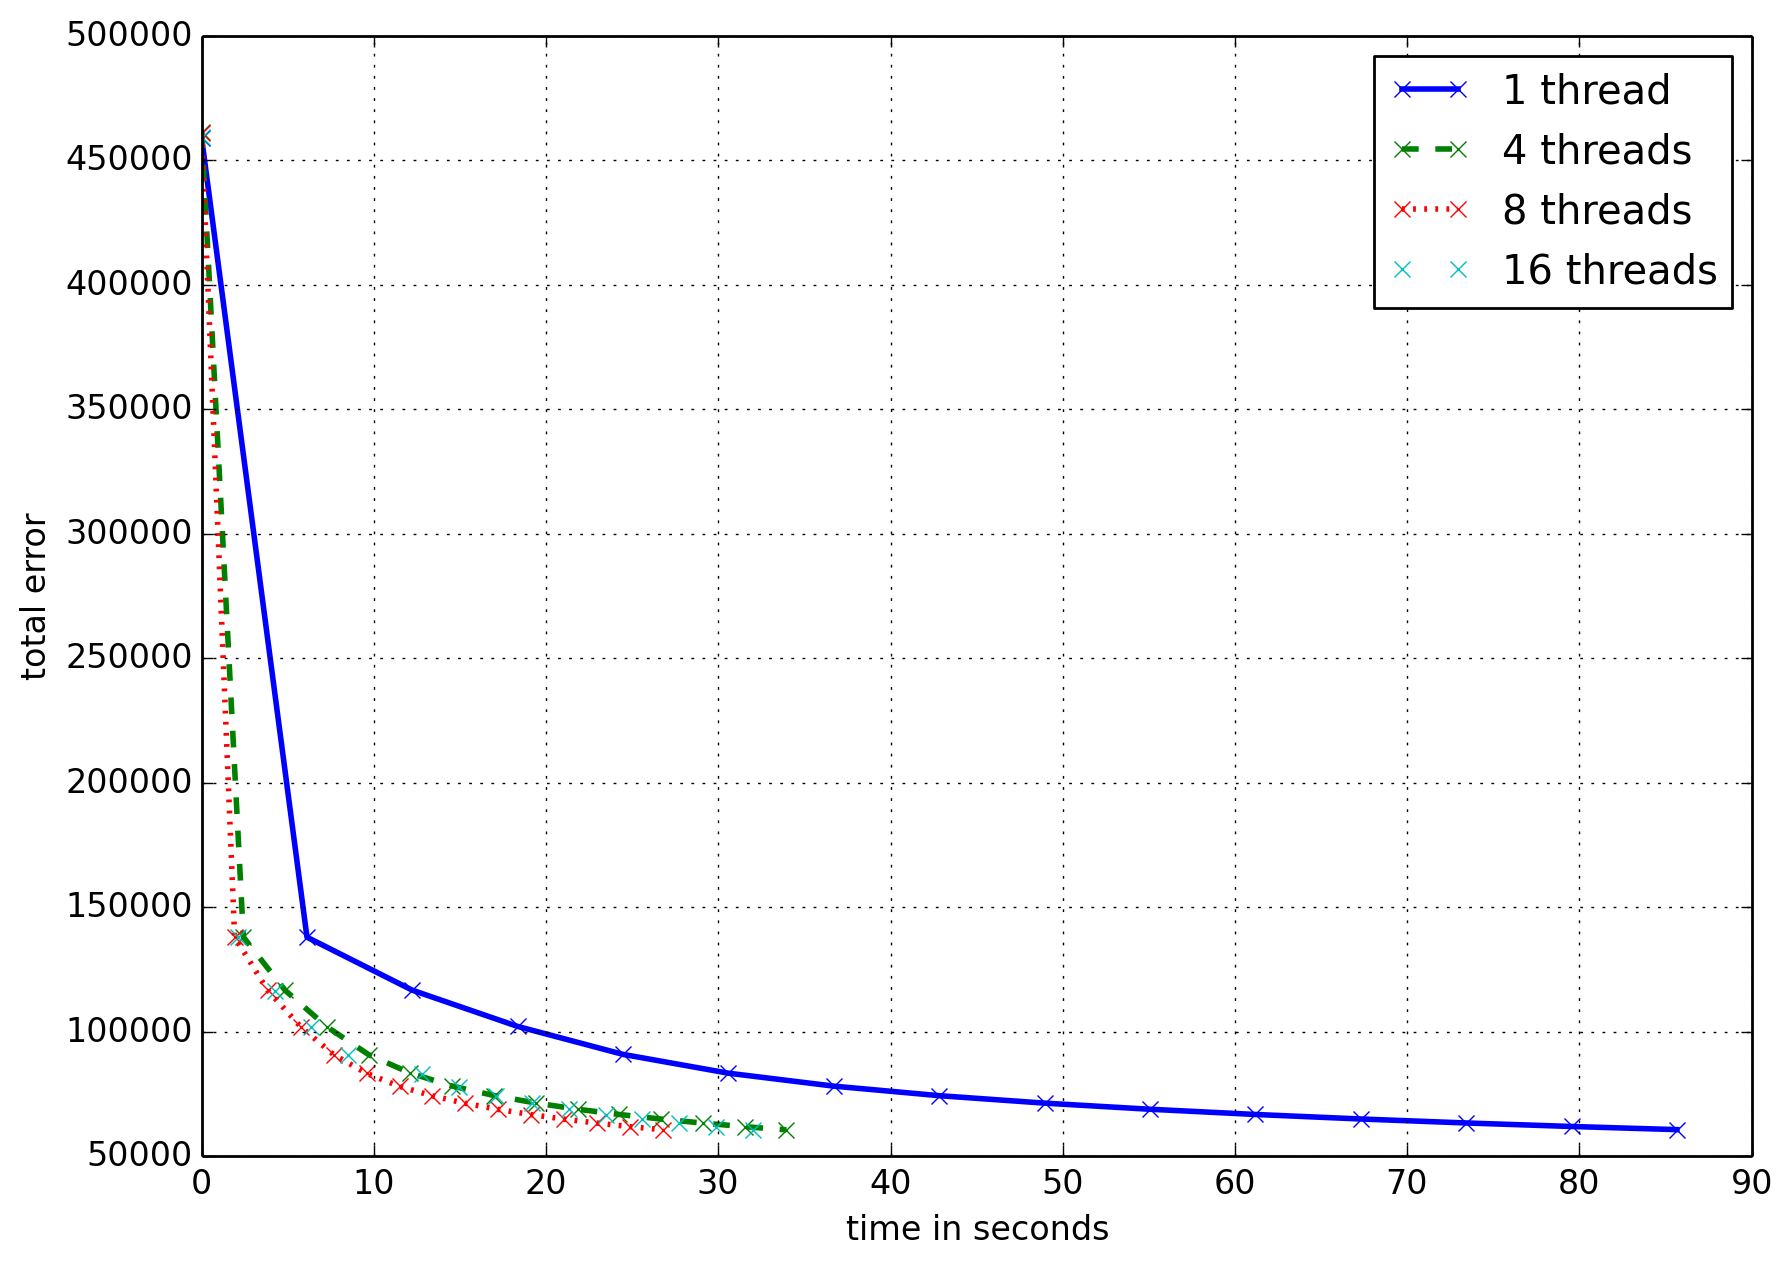
\includegraphics[width=0.7\linewidth]{experiment1SGD.png}
		\caption{Performance results on a single autoencoder layer with 500 hidden nodes and trained for 15 iterations. Plot shows time elapsed versus total training error over 5000 images for 1, 4, 8, and 16 threads.}
		\label{fig:experiment1}
	\end{figure}

\end{frame}


%%%%%%%%%%%%%%%%%%%%%%%%%%%%%%%%%%%%%
%% Frame
%%%%%%%%%%%%%%%%%%%%%%%%%%%%%%%%%%%%%%
\begin{frame}[t]
	\frametitle{Experimental Results: SGD Performance}
	\framesubtitle{~~}  %% needed for proper positioning of the logo ...

	\begin{figure}[h]
		\centering
		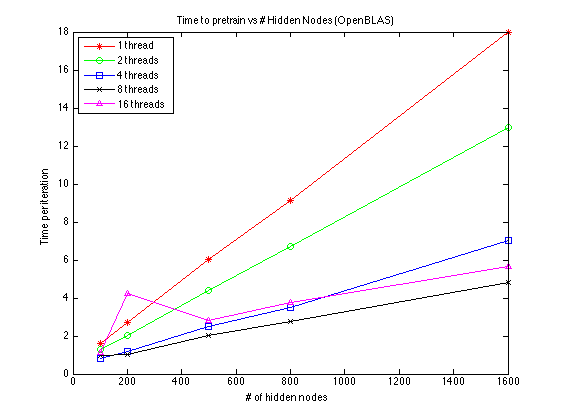
\includegraphics[width=0.7\linewidth]{performanceblas.png}
		\caption{Time per iteration versus the number of threads and hidden nodes. We parallelize with OpenBLAS and we use 5000 training images.}
		\label{fig:performanceblas}
	\end{figure}

\end{frame}


%%%%%%%%%%%%%%%%%%%%%%%%%%%%%%%%%%%%%
%% Frame
%%%%%%%%%%%%%%%%%%%%%%%%%%%%%%%%%%%%%%
\begin{frame}[t]
	\frametitle{Experimental Results: GA Performance}
	\framesubtitle{~~}  %% needed for proper positioning of the logo ...

	\begin{figure}[h] \centering
		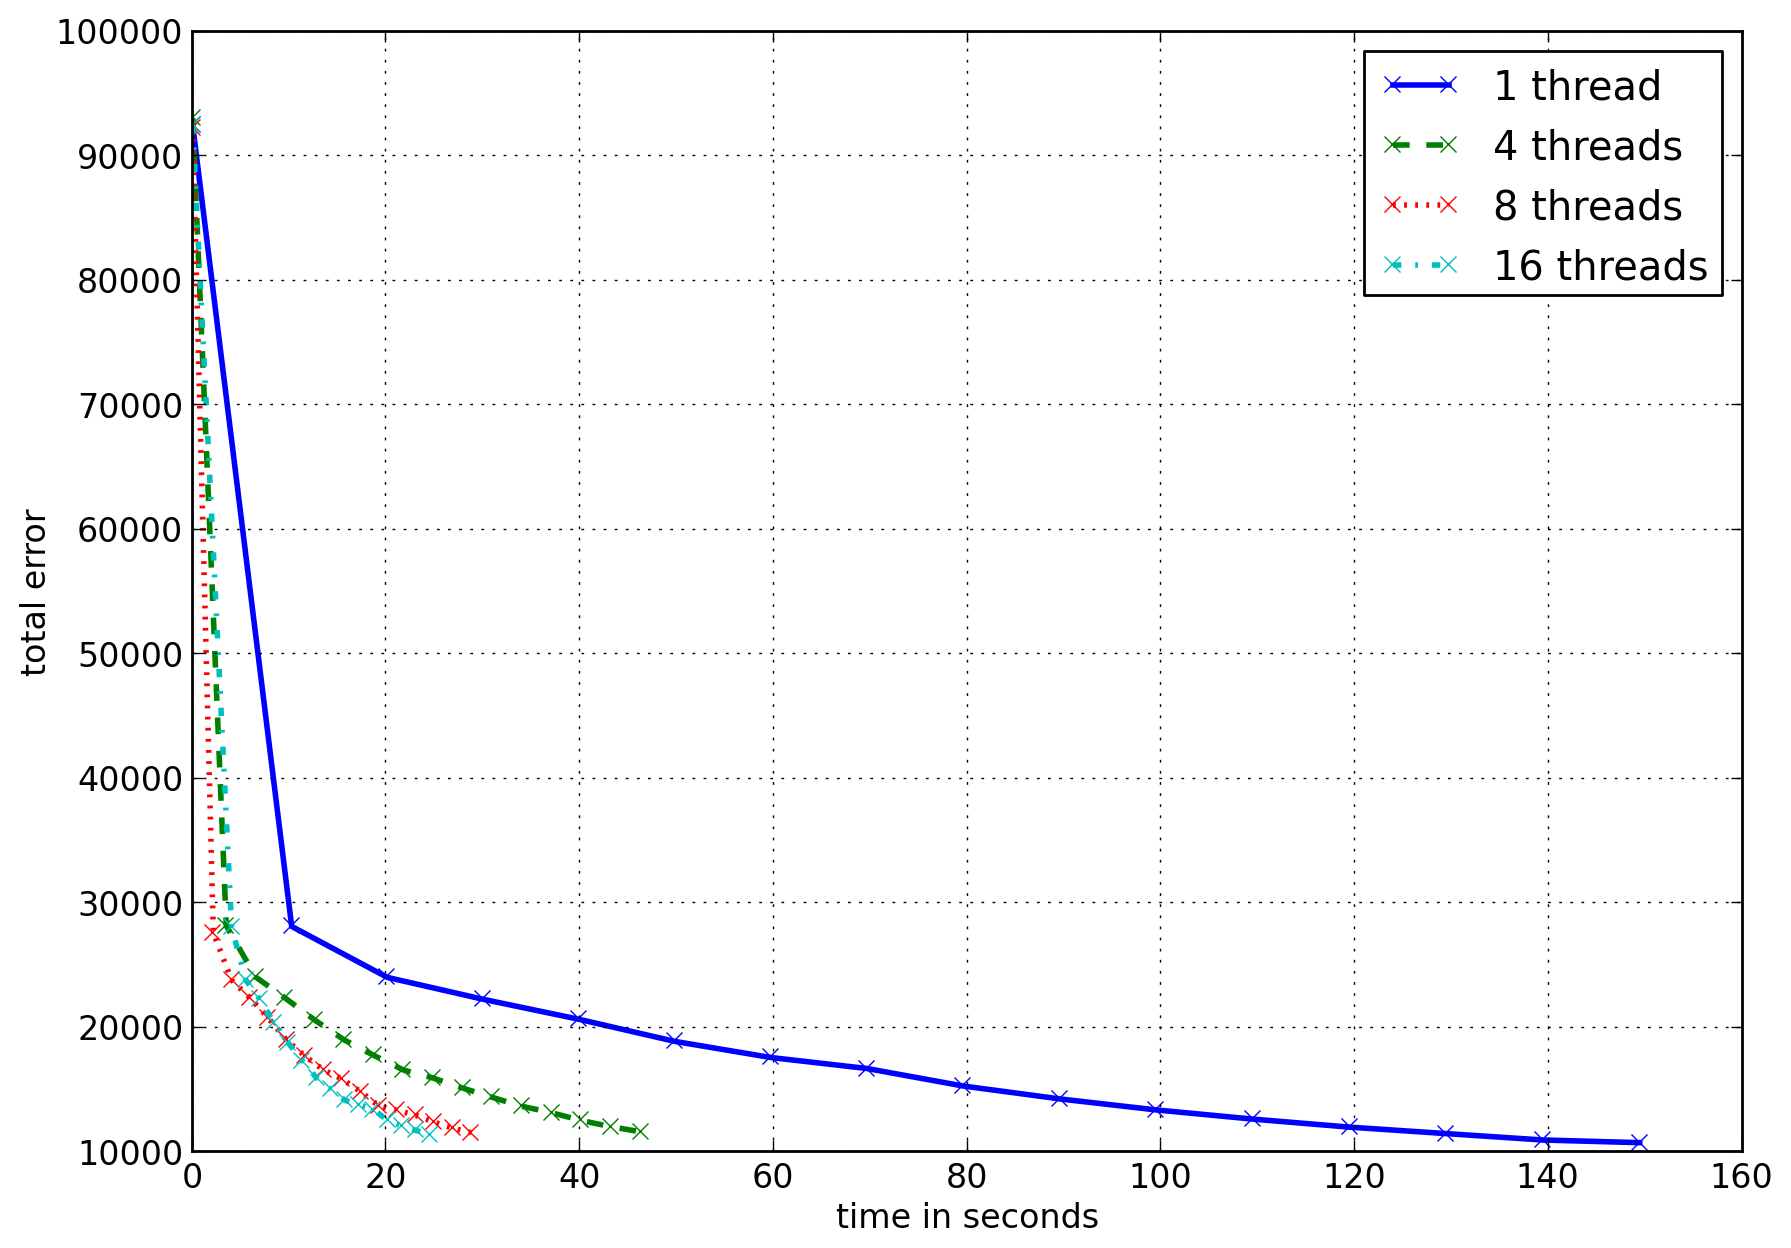
\includegraphics[width=0.7\linewidth]{ga_comparison2.png}
		\caption{Performance of HGA for 1, 4, 8, and 16 threads.}
		\label{fig:ga_comparison2}
	\end{figure}


\end{frame}


%%%%%%%%%%%%%%%%%%%%%%%%%%%%%%%%%%%%%
%% Frame
%%%%%%%%%%%%%%%%%%%%%%%%%%%%%%%%%%%%%%
\begin{frame}[t]
	\frametitle{Experimental Results: GA Performance}
	\framesubtitle{~~}  %% needed for proper positioning of the logo ...

\begin{figure}[H]
  \centering
  \subfloat[]{
    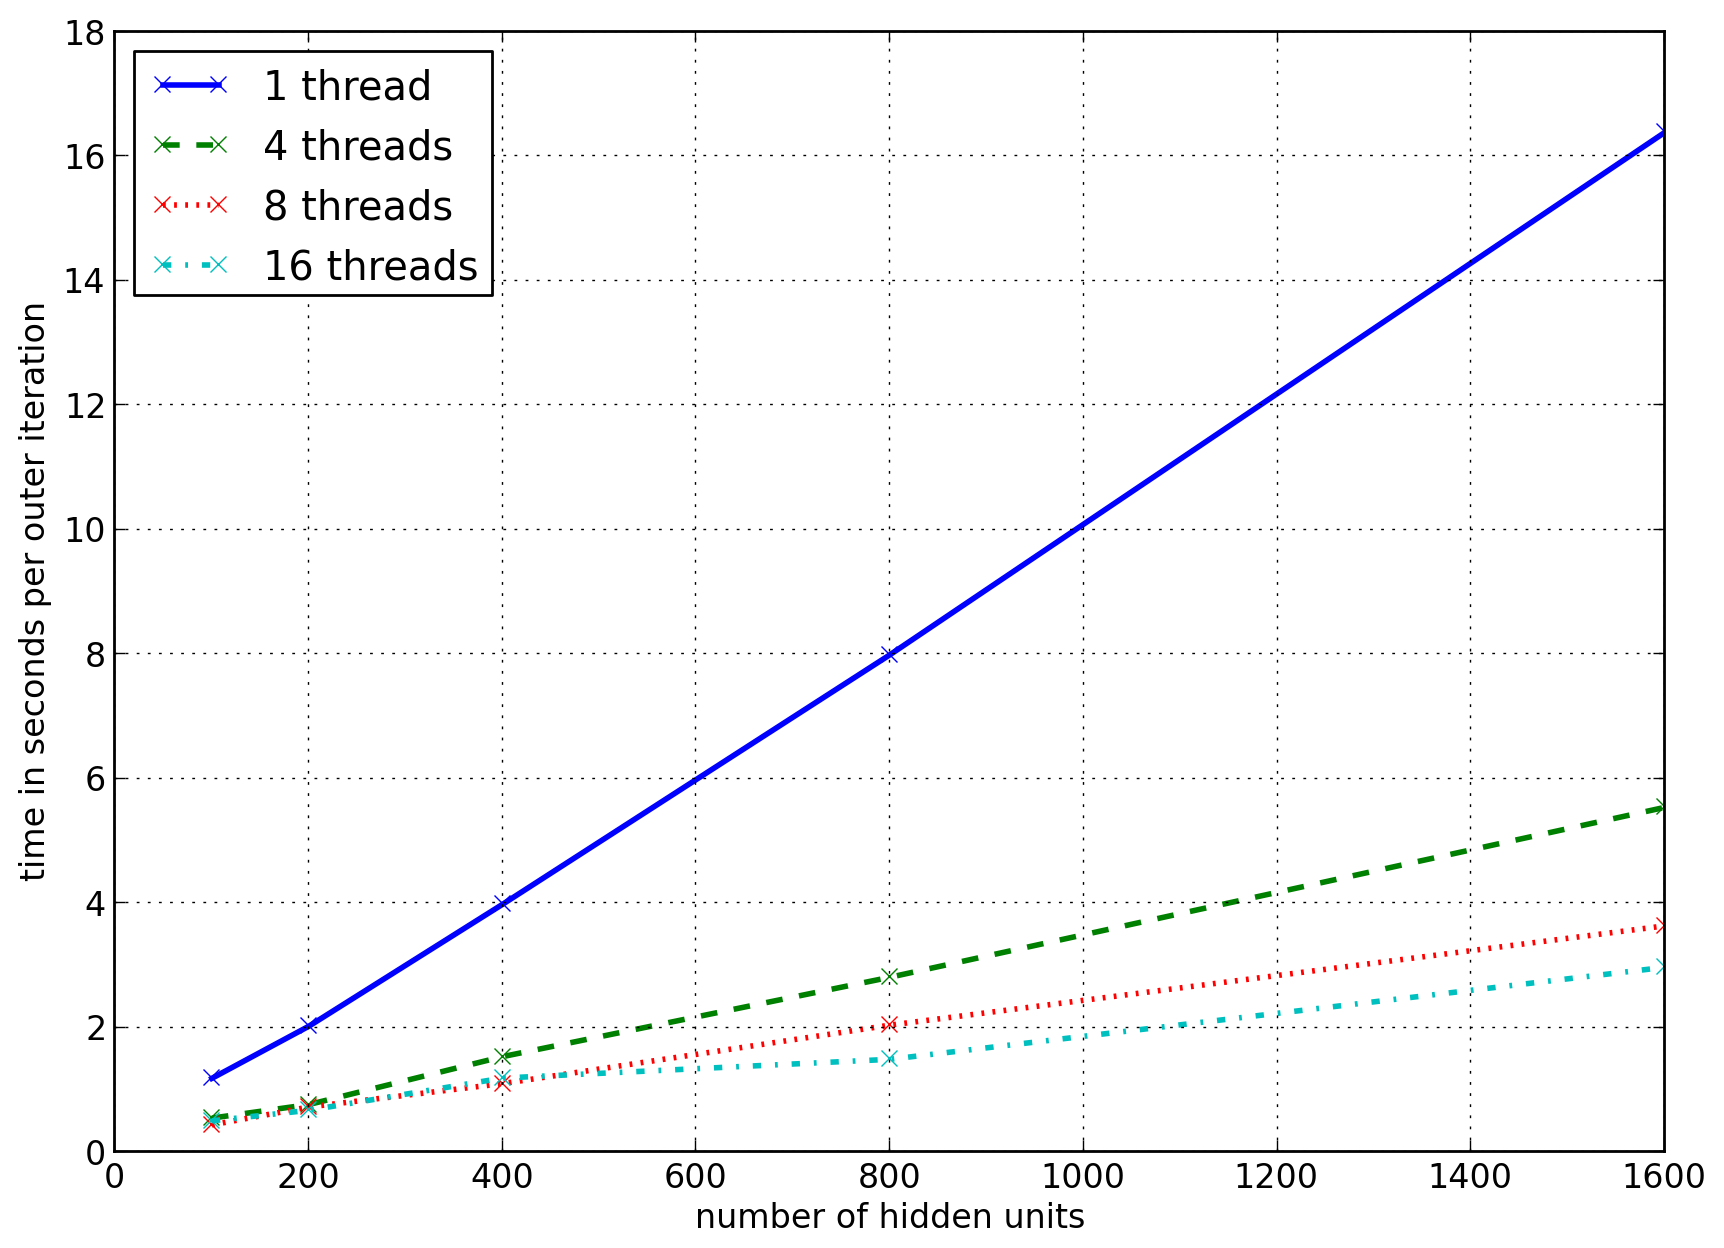
\includegraphics[width=0.4\textwidth]{ga_comparison3.png}
  }
  \subfloat[]{
    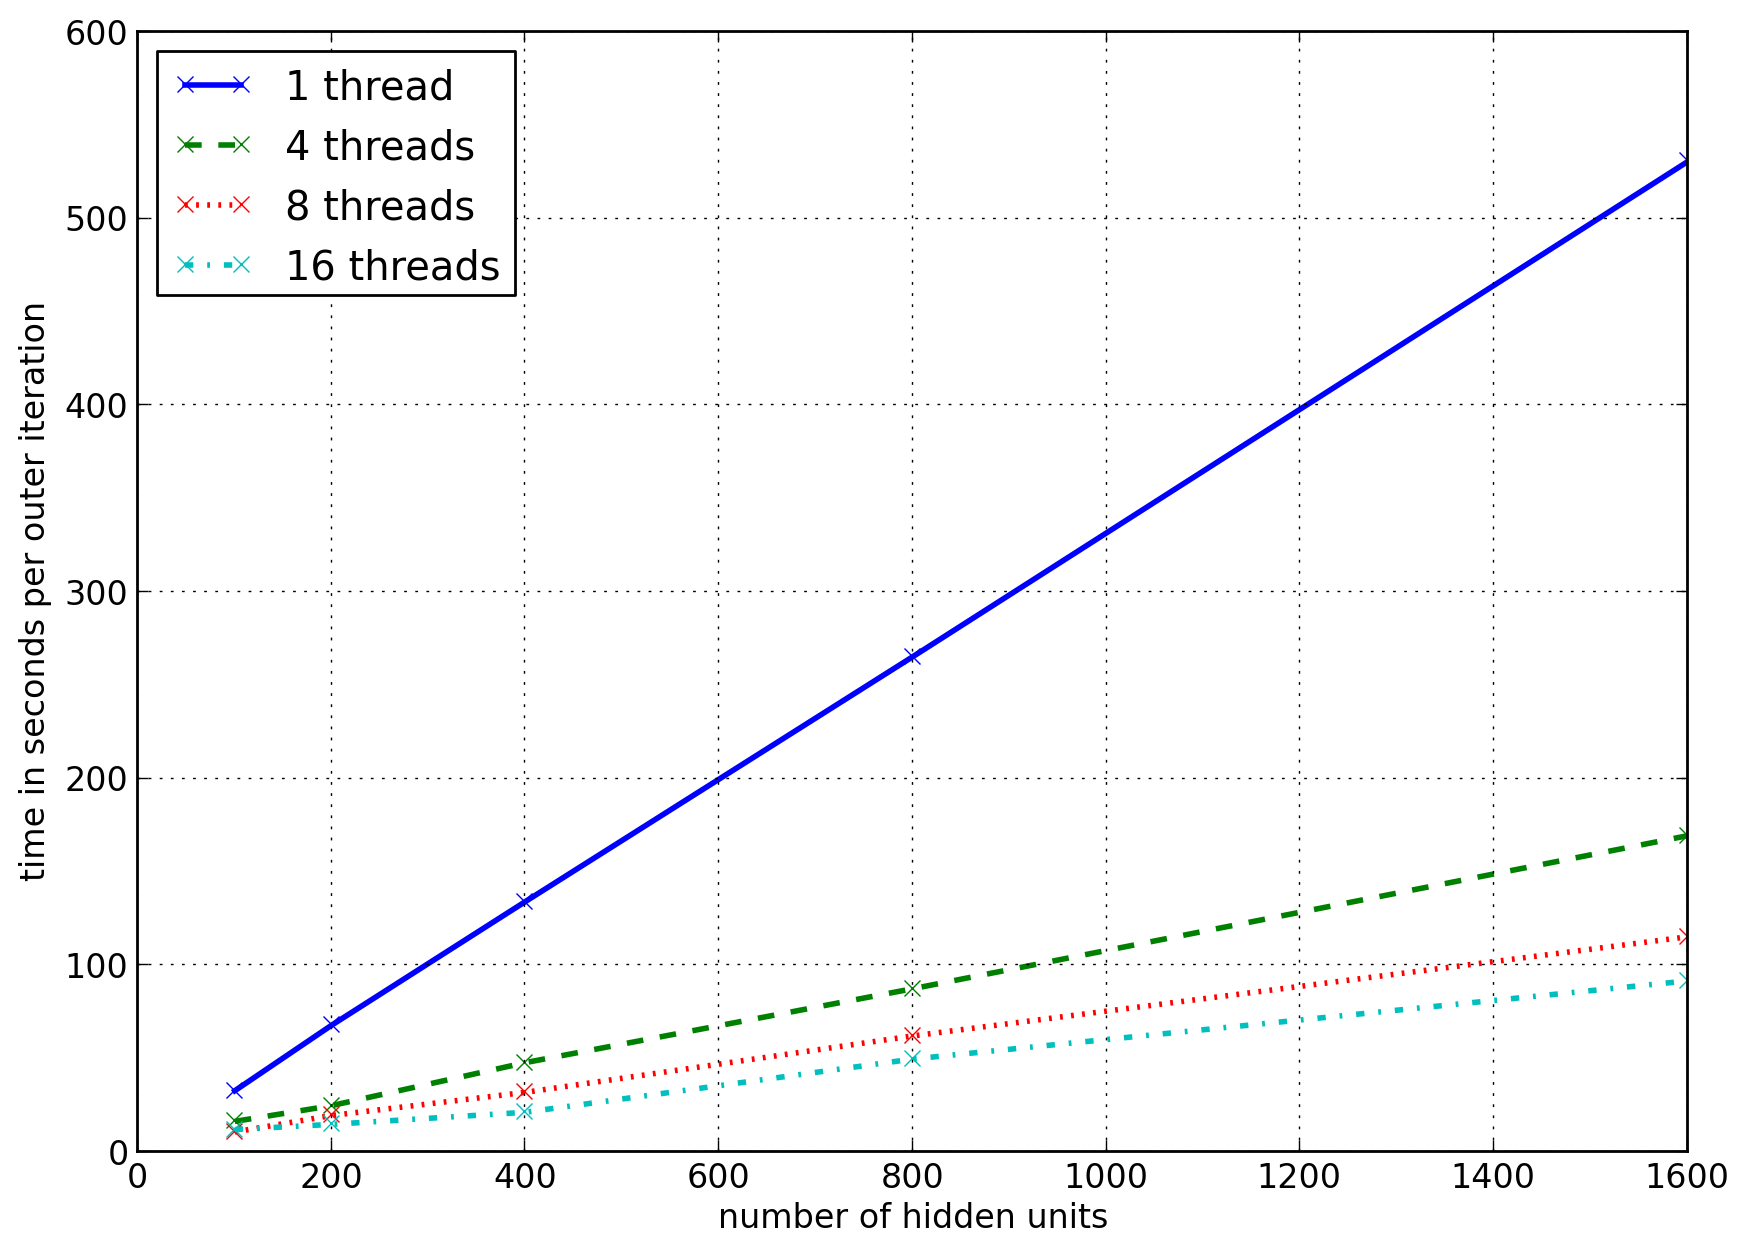
\includegraphics[width=0.4\textwidth]{ga_comparison3_big.png}
  }
  \caption{Comparison of performance versus number of threads and number of hidden units in autoencoder layer for HGA with population size (a) 2 and (b) 50.}
  \label{fig:ga_comparison3}
\end{figure}


\end{frame}


%%%%%%%%%%%%%%%%%%%%%%%%%%%%%%%%%%%%%
%% Frame
%%%%%%%%%%%%%%%%%%%%%%%%%%%%%%%%%%%%%%
\begin{frame}[t]
	\frametitle{Experimental Results: GA vs SGD Performance}
	\framesubtitle{~~}  %% needed for proper positioning of the logo ...

\begin{figure}[h] \centering
  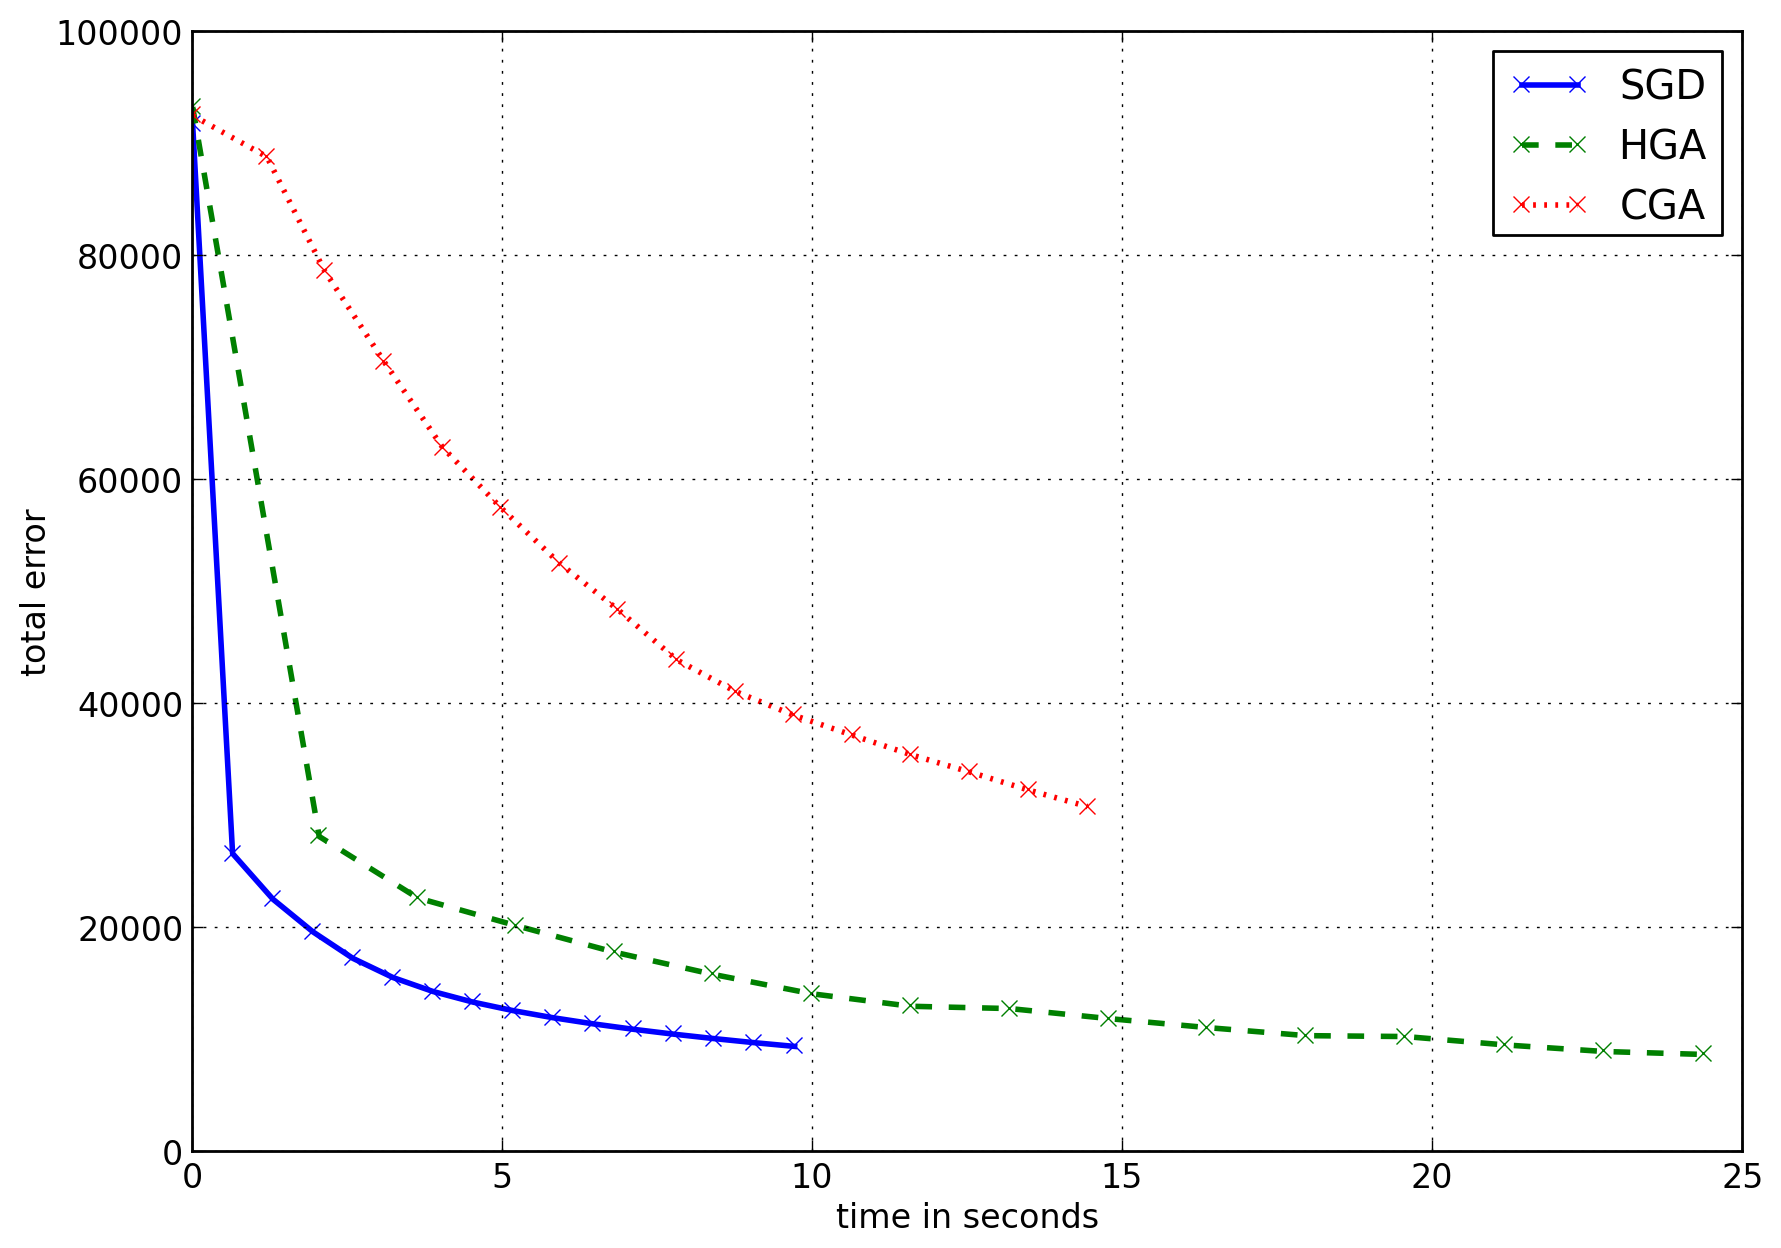
\includegraphics[width=0.7\linewidth]{ga_comparison.png}
  \caption{Comparison of the performance of SGD, HGA, and CGA. SGD is fastest, while HGA achieves the lowest reconstruction error.}
  \label{fig:ga_comparison}
\end{figure}

\end{frame}
